\chapter{Results and Discussion}
\label{ch:results_discussion}


\section{Size of codebase}
\label{sect:complexity}


\section{Test coverage}
\label{sect:test_coverage}

Testing is a great practice to guide the development and programming effort while conducting a software project, but it is of equal importance as a documentation tool allowing the technical staff to demonstrate to their clients (customers and managers alike) the care they exercised in constructing their codebase. Coverage testing detects if parts of the codebase were either just partly tested or not tested at all, taking into account LOC coverage, percentage of functions / methods invoked as well as branch or general statement coverage.

As can be seen in Figure~\ref{fig:test_coverage}, Graphinius JS has been exhaustively tested, reaching 100\% coverage for all but the branches department. The lower value in this section is a result of \textit{else-branches} not taken, in cases when there was no \textit{else-branch} to take. This can be remedied by re-writing all \textit{if-statements} in the form of \textit{(boolean condition \&\& consequent)}, so that the code coverage tool does not recognize the \textit{if} keyword. The author has successfully tested this practice on the PFS.ts file (as can be seen in Figure~\ref{fig:test_coverage}) but at the time of this writing considers it inappropriate to alter perfectly good code throughout the library just for the sake of artificially achieving 100\% coverage.

\begin{figure}[ht]
	% \centering
	\hspace*{-0.5cm}
	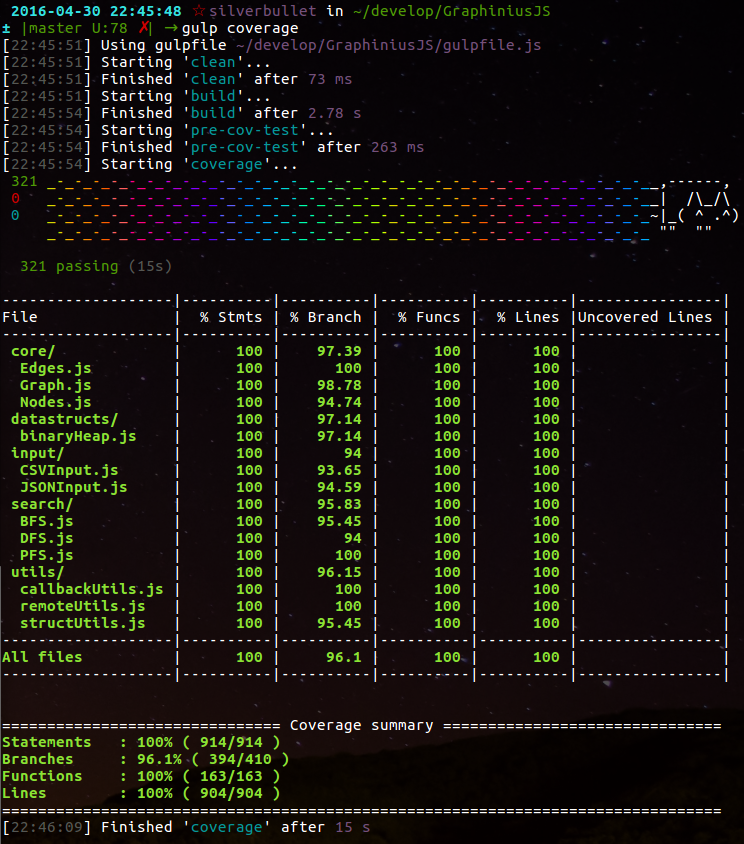
\includegraphics[width=1.1\textwidth]{figures/test_coverage}
	\caption{GraphiniusJS test coverage}
	\label{fig:test_coverage}
\end{figure}


\section{Performance compared to selected libraries}
\label{sect:perf_other_libs}

	\subsection{iGraph (c++)}
	\label{ssect:perf_igraph}
	
	\subsection{Graph Tool}
	\label{ssect:perf_graphtool}
	
	\subsection{NetworkX (pure python)}
	\label{ssect:perf_networkx}
	
	\subsection{Graphinius JS}
	\label{ssect:perf_graphinius}
	

\section{Execution speed in various scenarios}
\label{sect:performance}

	\subsection{graph loading}
	\label{ssect:perf_graph_loading}
	
	\subsection{degree distribution}
	\label{ssect:perf_deg_dist}
	
	\subsection{BFS / DFS}
	\label{ssect:perf_bfs_dfs}
	
	The test was performed on a graph of 


\section{Discussion of results}
\label{sect:discussion}
	